\begin{enumerate}[label=\thesubsection.\arabic*.,ref=\thesubsection.\theenumi]
	\item Determine the loop currents in 
    \figref{fig:ckt1}. 
		\begin{figure}[H] 
    \centering
    %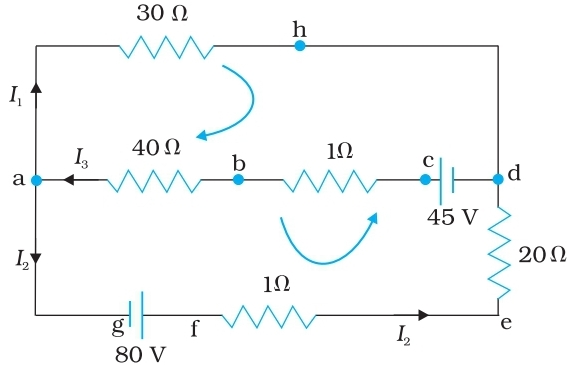
\includegraphics[width=\columnwidth]{figs/ckts/ckt1.jpg} % Adjust width or use height
    \resizebox{0.75\columnwidth}{!}{
	    \iffalse
\let\negmedspace\undefined
\let\negthickspace\undefined
\documentclass[journal,12pt,twocolumn]{IEEEtran}
\usepackage{cite}
\usepackage{amsmath,amssymb,amsfonts,amsthm}
\usepackage{algorithmic}
\usepackage{graphicx}
\usepackage{textcomp}
\usepackage{xcolor}
\usepackage{txfonts}
\usepackage{listings}
\usepackage{enumitem}
\usepackage{mathtools}
\usepackage{gensymb}
\usepackage{comment}
\usepackage[breaklinks=true]{hyperref}
\usepackage{tkz-euclide} 
\usepackage{listings}
\usepackage{gvv}                                        
%\def\inputGnumericTable{}                                 
\usepackage[latin1]{inputenc}                                
\usepackage{color}                                            
\usepackage{array}                                            
\usepackage{longtable}                                       
\usepackage{calc}                                             
\usepackage{multirow}                                         
\usepackage{hhline}                                           
\usepackage{ifthen}                                           
\usepackage{lscape}
\usepackage{tabularx}
\usepackage{array}
\usepackage{float}
\usepackage{circuitikz}

\newtheorem{theorem}{Theorem}[section]
\newtheorem{problem}{Problem}
\newtheorem{proposition}{Proposition}[section]
\newtheorem{lemma}{Lemma}[section]
\newtheorem{corollary}[theorem]{Corollary}
\newtheorem{example}{Example}[section]
\newtheorem{definition}[problem]{Definition}
\newcommand{\BEQA}{\begin{eqnarray}}
\newcommand{\EEQA}{\end{eqnarray}}
\newcommand{\define}{\stackrel{\triangle}{=}}
\theoremstyle{remark}
\newtheorem{rem}{Remark}

% Marks the beginning of the document
\begin{document}
\bibliographystyle{IEEEtran}
\vspace{3cm}

\renewcommand{\thefigure}{\theenumi}
\renewcommand{\thetable}{\theenumi}
\fi


\begin{circuitikz}

\draw (8,0) to [resistor, l_ = $1 \Omega$, color=cyan] (4,0) to [battery1, l=$80 V$, color=cyan] (0,0);

\draw (8,0) to [resistor, l_ = $20 \Omega$, color=cyan] (8,2);
\draw (6,2) to [battery1, l_= $45 V$, color=cyan] (8,2);
\draw (6,2) to [resistor, l_ = $1 \Omega$, color=cyan] (4,2) to [resistor, l_ = $40 \Omega$, color=cyan] (1,2) to [short](0,2);

\draw (0,0) to [short] (0,4);
\draw (0,4) to [resistor, l = $30 \Omega$, color=cyan](6,4);
\draw (6,4) to [short](8,4);
\draw (8,4) to [short](8,2);

% Writing nodes
\draw (0,2) node[label={left:a}, circ, color=cyan]{};
\draw (3.75,2) node[label={above:b}, circ, color=cyan]{};
\draw (6.5,2) node[label={above:c}, circ, color=cyan]{};
\draw (8,2) node[label={right:d}, circ, color=cyan]{};
\draw (0,2) node[label={left:a}, circ, color=cyan]{};
\draw (8,0) node[label={right:e}]{};
\draw (5,0) node[label={below:f}]{};
\draw (1.5,0) node[label={below:g}]{};
\draw (6,4) node[label={above:h}, circ, color=cyan]{};
\draw[->,shift={(4,3)},color=cyan] (120:.7cm) arc (120:-90:.7cm) node at(0,0){$I_1$};
\draw[->,shift={(4,1)},color=cyan] (120:.7cm) arc (120:-90:.7cm) node at(0,0){$I_2$};

\end{circuitikz}

%\end{document}
 % Adjust width or use height
    }
    \caption{} 
    \label{fig:ckt1} 
\end{figure}
	\item Determine the current in each branch of the network shown in 
    \figref{fig:ckt2}. 
		\begin{figure}[H] 
    \centering
    \resizebox{0.75\columnwidth}{!}{
	    \iffalse
\documentclass{article}

\usepackage{tikz}
\usepackage{circuitikz}

\begin{document}

\begin{figure}[h!]
  \begin{center}
	  \fi
    \begin{circuitikz}
	    \draw[scale = 0.8] (0,0)
	    node[label={[font=\footnotesize]above:$A$}] {}
	to[battery1, l = { $10V$}, color = cyan, /tikz/circuitikz/bipoles/length=70pt] (4,0) 
	    to[R, l={ $1\Omega$}, color=cyan,/tikz/circuitikz/bipoles/length=70pt] (8,0)
	    node[label={[font=\footnotesize]right:$C$}] {}
	    to[R,l ={ $2\Omega$}, color = cyan,/tikz/circuitikz/bipoles/length=70pt] (8,4)
	    node[label={[font=\footnotesize]above:$B$}] {}
	    to[R,l={ $4\Omega$}, color = cyan,/tikz/circuitikz/bipoles/length=70pt] (0,0)
      to[R,l=$4\Omega$, color = cyan,/tikz/circuitikz/bipoles/length=70pt] (8,-4)
	    node[label={[font=\footnotesize]below:$D$}] {}
	    to[R,l={$2\Omega$}, color = cyan,/tikz/circuitikz/bipoles/length=70pt] (8,0);
	    \draw[scale =0.8] (8,-4)
      to[short] (12,0)
	    to[battery1,l={$5V$},invert, color = cyan] (12,0.5)
	    node[label={[font=\footnotesize]above:$\epsilon$}] {}
      to[short] (8,4);
\draw[->,shift={(5,1.5)}] (120:.7cm) arc (120:-90:.5cm) node at(0,0){$I_1$};
  \draw[->,shift={(7.5,0)}] (120:.7cm) arc (120:-90:.7cm) node at(0,0){$I_2$};
\draw[->,shift={(5,-1.5)}] (120:.7cm) arc (120:-90:.5cm) node at(0,0){$I_3$};
    \end{circuitikz}
    \iffalse
  \end{center}
\end{figure}

\end{document}
\fi
 % Adjust width or use height
    }
    %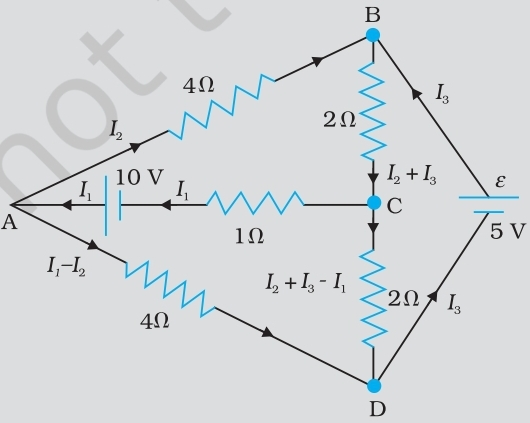
\includegraphics[width=\columnwidth]{figs/ckts/ckt2.jpg} % Adjust width or use height
    \caption{} 
    \label{fig:ckt2} 
\end{figure}
	\item In \figref{fig:ckt3}, a galvanometer of $15\ohm$ resistance is connected across BD. Calculate the current through the galvanometer when a potential difference of $10 V$ is maintained across AC.
		\begin{figure}[H] 
    \centering
    %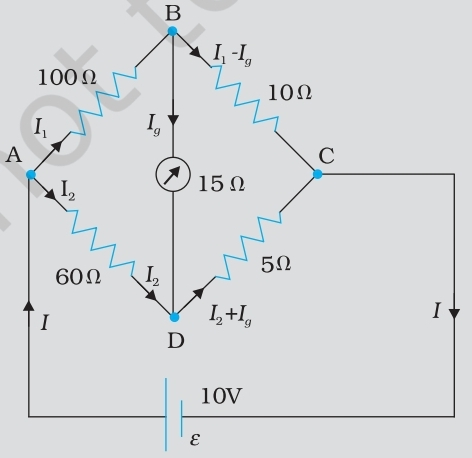
\includegraphics[width=\columnwidth]{figs/ckts/ckt3.jpg} % Adjust width or use height
    \resizebox{0.75\columnwidth}{!}{
	    \iffalse
\let\negmedspace\undefined
\let\negthickspace\undefined
\documentclass[journal,12pt,twocolumn]{IEEEtran}
\usepackage{cite}
\usepackage{amsmath,amssymb,amsfonts,amsthm}
\usepackage{algorithmic}
\usepackage{graphicx}
\usepackage{textcomp}
\usepackage{xcolor}
\usepackage{txfonts}
\usepackage{listings}
\usepackage{enumitem}
\usepackage{mathtools}
\usepackage{gensymb}
\usepackage{comment}
\usepackage[breaklinks=true]{hyperref}
\usepackage{tkz-euclide} 
\usepackage{listings}
\usepackage{gvv}                                        
%\def\inputGnumericTable{}                                 
\usepackage[latin1]{inputenc}                                
\usepackage{color}                                            
\usepackage{array}                                            
\usepackage{longtable}                                       
\usepackage{calc}                                             
\usepackage{multirow}                                         
\usepackage{hhline}                                           
\usepackage{ifthen}                                           
\usepackage{lscape}
\usepackage{tabularx}
\usepackage{array}
\usepackage{float}
\usepackage{tikz}
\usepackage{circuitikz}

\newtheorem{theorem}{Theorem}[section]
\newtheorem{problem}{Problem}
\newtheorem{proposition}{Proposition}[section]
\newtheorem{lemma}{Lemma}[section]
\newtheorem{corollary}[theorem]{Corollary}
\newtheorem{example}{Example}[section]
\newtheorem{definition}[problem]{Definition}
\newcommand{\BEQA}{\begin{eqnarray}}
\newcommand{\EEQA}{\end{eqnarray}}
\newcommand{\define}{\stackrel{\triangle}{=}}
\theoremstyle{remark}
\newtheorem{rem}{Remark}

% Marks the beginning of the document
\begin{document}
\bibliographystyle{IEEEtran}
\renewcommand{\thefigure}{\theenumi}
\renewcommand{\thetable}{\theenumi}
\fi
\begin{circuitikz}
   
    \draw (0,0)--(0,4) node[label={[font=\footnotesize]left:A},color=cyan]{}
    to[resistor,i=$ $,l=$100 \Omega$, color=cyan,*-*] (2,6) node[label={[font=\footnotesize]above:B}]{}
    to[resistor,i= $ $,l=$10 \Omega$,color=cyan,*-*] (4,4) node[label={[font=\footnotesize]above:C}]{}
    ;
    \draw (0,4) to[resistor,i=$ $,l_=$60 \Omega$,color=cyan,*-*] (2,2) node[label={[font=\footnotesize]below:D}]{}
    to[resistor,i=$ $,l_=$5 \Omega$,color=cyan,*-*] (4,4)
    
    ;
    \draw (4,4)--(6,4)--(6,0) 
    ;
    \draw (0,0) to[battery1, i= $ $,l=$10V$,color=cyan] (6,0)
    ;
    \draw (2,6)--(2,4.5);
    \draw (2,3.5)--(2,2);
    \draw[thick,->] (1.7,3.7)--(2.3,4.3);
    \draw (2,4) circle (0.5); 
    \node at (3,4) {$15\Omega$};
    \node at (3,-0.75) {$\epsilon$};
\end{circuitikz}

%\end{document}
 % Adjust width or use height
    }
    \caption{} 
    \label{fig:ckt3} 
\end{figure}
	\item Determine the current in each branch of the network shown in 
\figref{fig:ckt4}.
		\begin{figure}[H] 
    \centering
    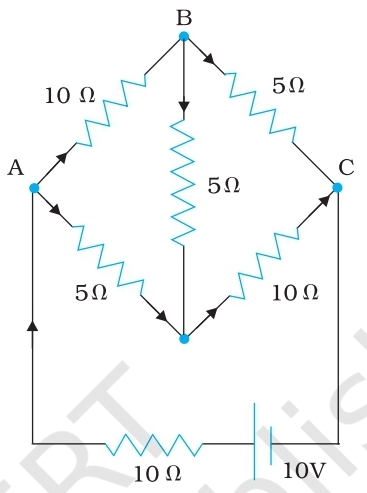
\includegraphics[width=\columnwidth]{figs/ckts/ckt4.jpg} % Adjust width or use height
    \caption{} 
    \label{fig:ckt4} 
\end{figure}
\end{enumerate}
 

